\begin{figure*}[t]
\centering
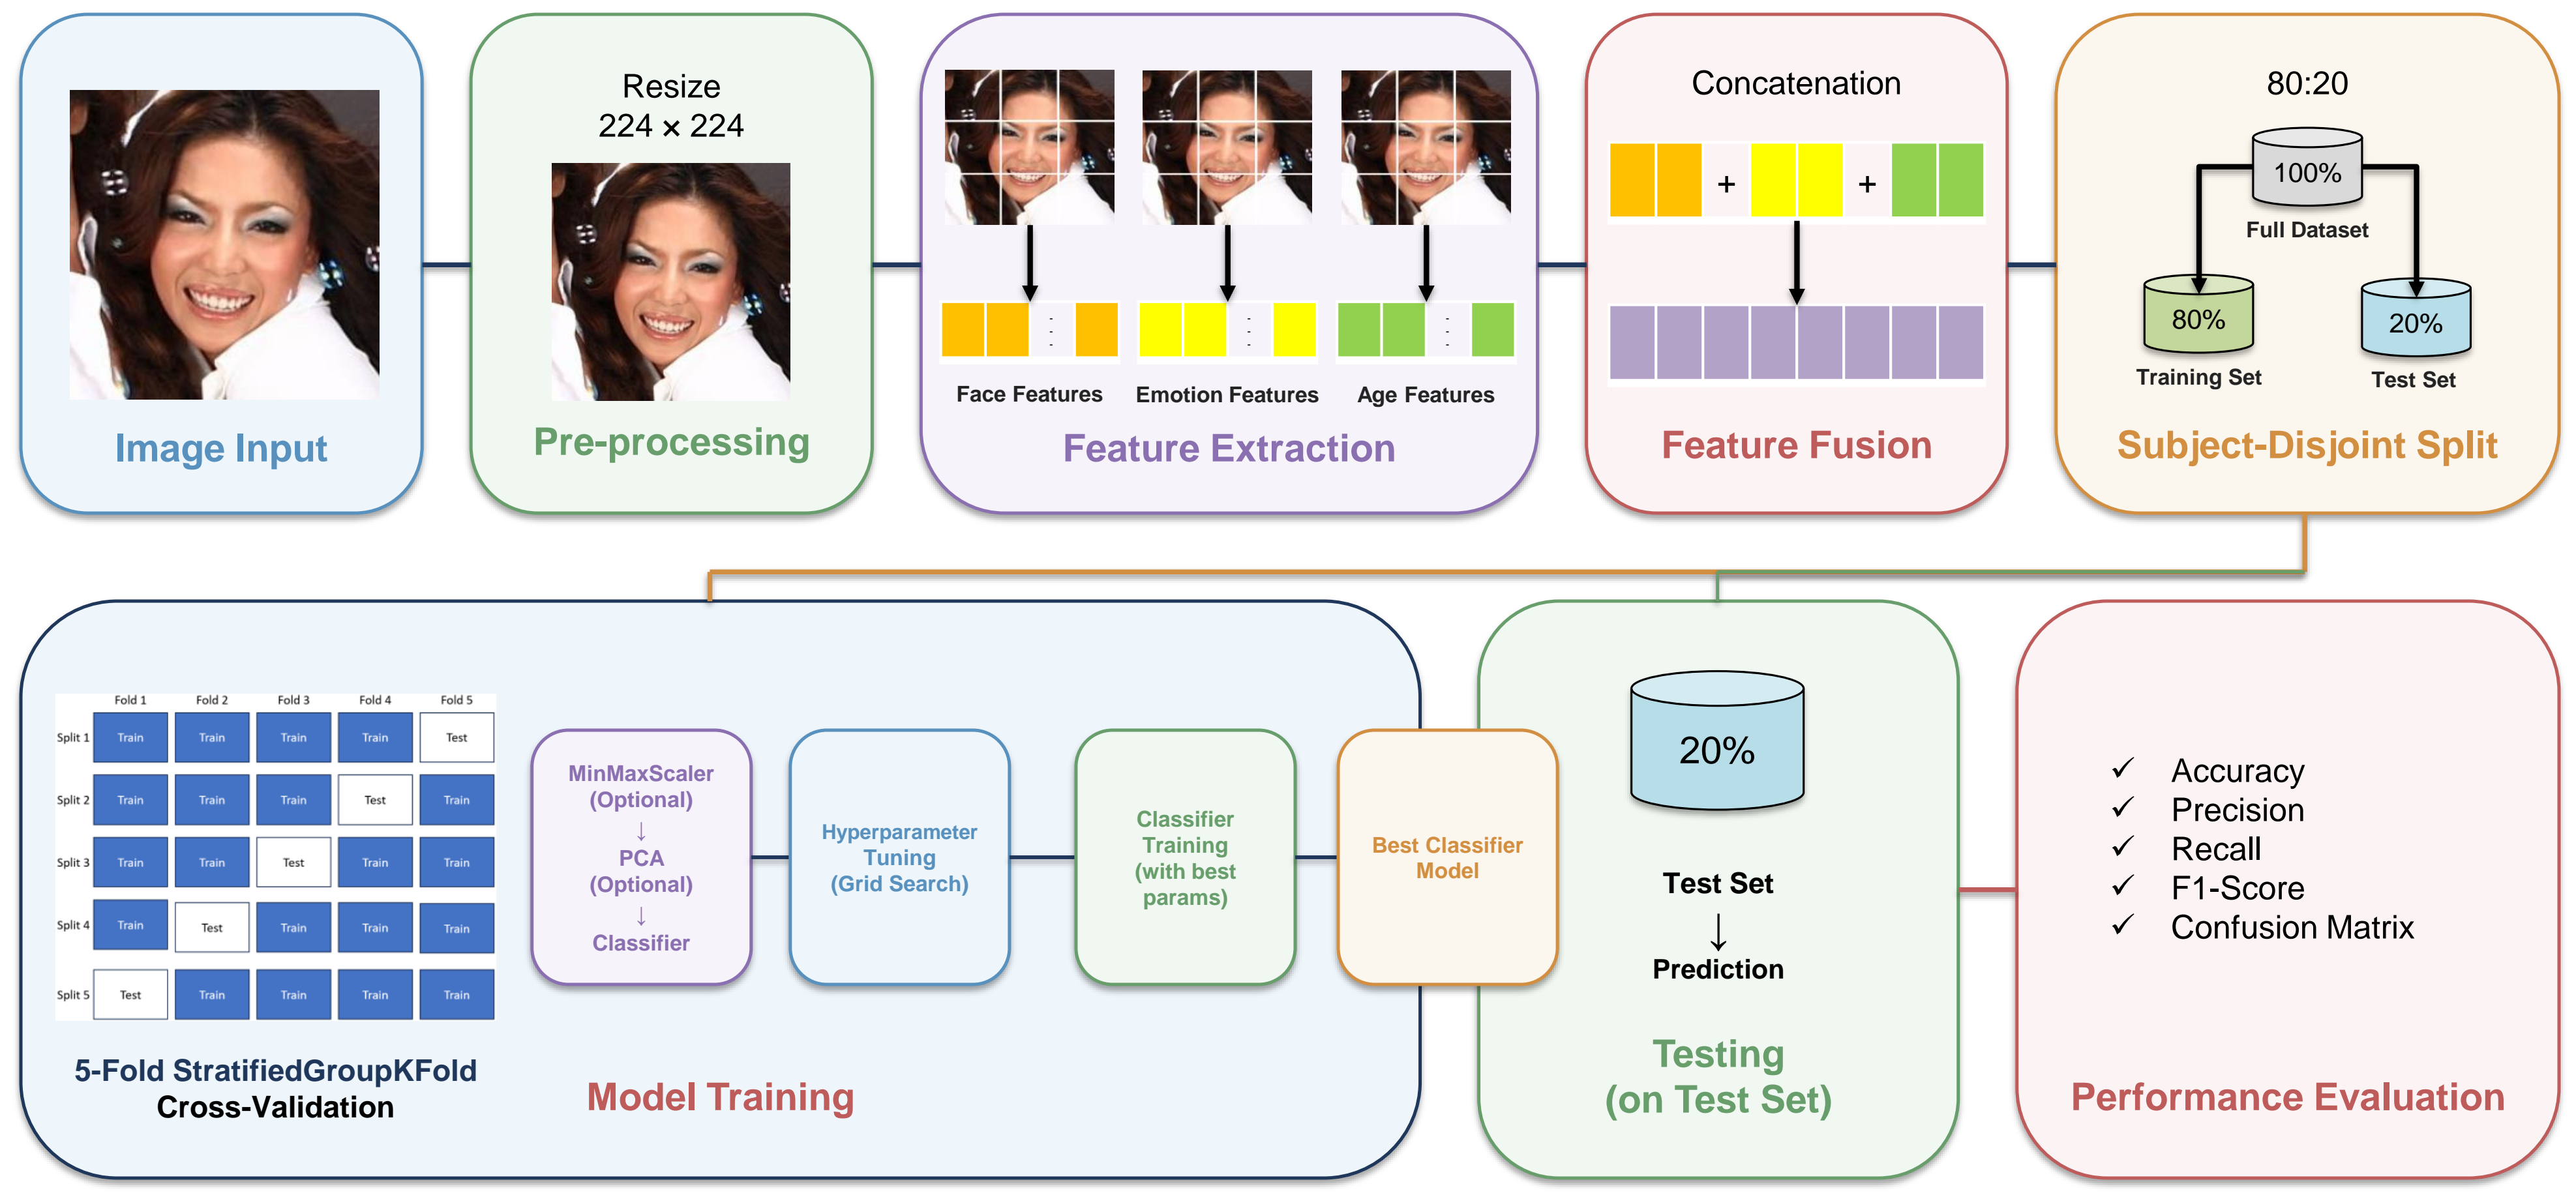
\includegraphics[width=\textwidth]{method_v2.png}
\caption{End-to-End Framework of the Proposed Multi-Domain Vision Transformer Feature Fusion and Classical Classifier Optimization for Intersectional Race and Gender Classification.}
\label{fig:1}
\end{figure*}

\section{Materials and Methods}
\label{sec:materials_and_methods}

The end-to-end computational framework proposed in this study is designed to classify intersectional race and gender in a unified manner, as illustrated in Figure~\ref{fig:1}. The methodological pipeline begins with raw DemogPairs facial image inputs strictly partitioned through the Strict Subject-Disjoint Partitioning protocol (80\% training set and 20\% held-out test set) to guarantee the absolute elimination of subject identity leakage. Subsequently, each facial image is processed by three task-specific ViT models frozen offline to extract high-dimensional multi-domain latent representations, encompassing facial biometric craniofacial geometric features, dynamic affective emotion expression patterns, and biological aging morphological markers. These three 768-dimensional latent representations are unified through a direct concatenation fusion operation to form a 2,304-dimensional tri-domain joint representation vector. This fused vector is then fed into a chained modular processing pipeline optimized via 5-Fold StratifiedGroupKFold Grid Search Cross-Validation (GridSearchCV) at the isolated fold level to classify the six demographic subgroups objectively and without bias.
